\documentclass{article}

\usepackage{tikz}
\usetikzlibrary{mindmap,trees}
\begin{document}
\pagestyle{empty}
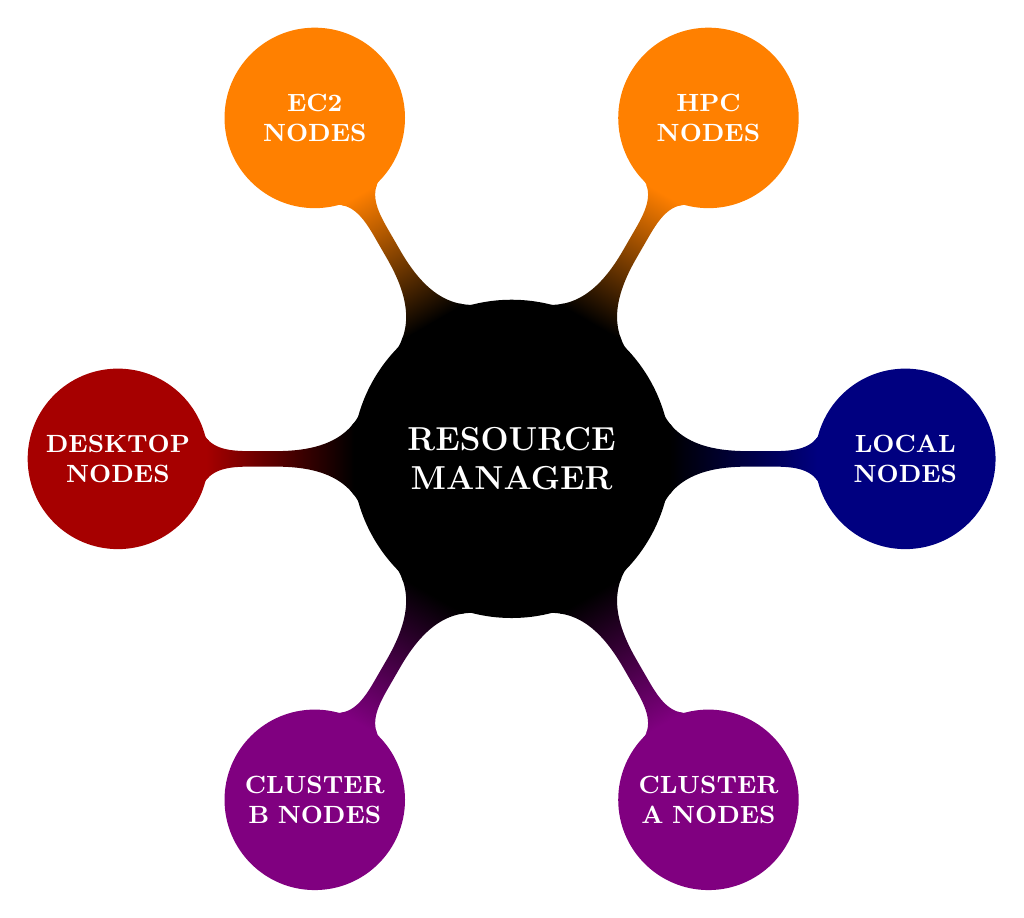
\begin{tikzpicture}
  \path[mindmap,concept color=black,text=white]
  node[concept] {\textbf{RESOURCE MANAGER}}
    [clockwise from=0]
    child[concept color=blue!50!black] { node[concept] {\textbf{LOCAL NODES}} }  
    child[concept color=violet] { node[concept] {\textbf{CLUSTER A NODES}} }  
    child[concept color=violet] { node[concept] {\textbf{CLUSTER B NODES}} }
    child[concept color=red!65!black] { node[concept] {\textbf{DESKTOP NODES}} }
    child[concept color=orange] { node[concept] {\textbf{EC2 NODES}} }
    child[concept color=orange] { node[concept] {\textbf{HPC NODES}} }
    %child[concept color=green!50!black] { node[concept] {Dataserver} }
    ;
\end{tikzpicture}\end{document}
